\documentclass{article}
\usepackage{enumitem}
\usepackage{listings}
\usepackage{graphicx}
\usepackage{microtype}
\usepackage{amsmath}
\usepackage[utf8]{inputenc}
\documentclass{article}
\newcommand{\myskip}{\par\null\par}
\title{Math 305 Homework 4}
\author{Theodore Koss}
\date{April 2023}
\begin{document}

\maketitle
\section*{Problem 1}\begin{itemize}
    \item Colley Ratings: Where $C$ = Colley rating of a team\\
$W$ = number of wins by the team\\
$P$ = number of opponents the team has played\\
$G$ = number of games played by the team\\ \begin{itemize}
        \item $C_1=\frac{W_1+P_1}{2G_1}=\frac{5+3}{12}=.66$
        \item $C_2=\frac{W_2+P_2}{2G_2}=\frac{3+3}{12}=.5$
        \item $C_3=\frac{W_3+P_3}{2G_3}=\frac{3+3}{12}=.5$
        \item $C_4=\frac{W_4+P_4}{2G_4}=\frac{1+3}{12}=.33$
    \end{itemize}
    \item Massey Ratings: (Not sure)
\end{itemize}
\section*{Problem 2}
Experienced chess players A and B both start with a rating of 2600. They play two
games, first A beats B, then B beats A. Will the rating of A equal the rating of B after
these two games? Should the ratings be equal? Describe your thoughts.\par\null\par No, the ratings would not be equal, because although they begin at the same place, after player A beats B, their rating goes up, whereas player B's rating goes down. Therefore, for the next game, when player B wins, they are beating a higher rated player, therefore gaining more elo than if they were both the same.
\section*{Problem 3}
Two chess players have Elo ratings that differ by 400n, where n is a non-negative
integer. How likely is the higher rated player to win for different values of n? How
much more likely is the higher rated player to win than the lower rated one for
different values of n? (Consider n = 0, 1, 2, . . . 4 to see a pattern or analyze the
formula for win probability.)\begin{itemize}
    \item $n=0$, $P=50\%$
    \item $n=1$, $P=90.91\%$
    \item $n=2$, $P=99\%$
    \item $n=3$, $P=99.9\%$
    \item $n=4$, $P=99.99\%$
    \item $n=i$, $P=\frac{1}{1+10^{-i}}$
\end{itemize}
\section*{Problem 4}
Suppose a truck rental company has locations in Dallas, TX, Raleigh, NC and Miami, FL. The company permits one-way rentals and knows that based on previous
experience that during a typical week the following truck movements occur:
Of the trucks that start in Dallas:\begin{itemize}
    \item 50\% stay in Dallas
\item 25\% travel to Raleigh
\item 25\% travel to Miami
\end{itemize}
Of the trucks that start in Raleigh:\begin{itemize}
\item 40\% stay in Raleigh
\item 20\% travel to Dallas
\item 40\% travel to Miami
\end{itemize}
Of the trucks that start in Miami:\begin{itemize}
\item 80\% stay in Miami
\item 15\% travel to Dallas
\item 5\% travel to Raleigh
\end{itemize}
Draw a transition diagram for the model adding the given probabilities. If 150
trucks start in each city, use MATLAB to determine the long-term numbers of trucks
in each city (steady-state)\newline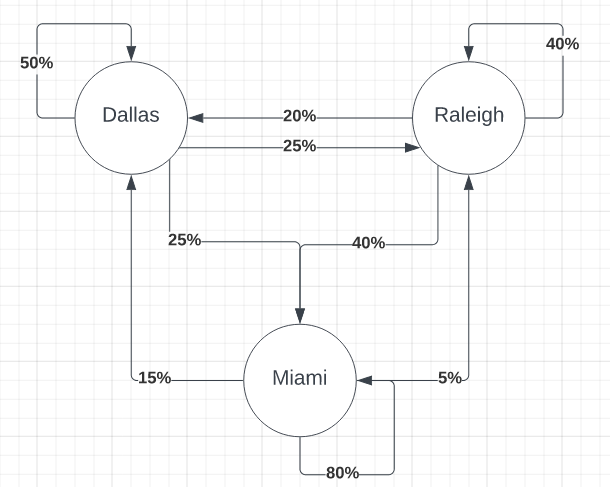
\includegraphics[scale=.5]{Pictures/image_2023-04-06_133826624.png} $$A=\begin{pmatrix}.5 & .25 & .25\\ .2 & .4 & .4 \\ .15 & .05 & .8\\
\end{pmatrix}$$ $$\lambda_1=1$$ $$v_1=(1\ 1\ 1)$$ Therefore all 3 cities will have 150 trucks as time goes on.
\end{document}